\subsection{What is a better forecast worth? Decision-focused evaluation}\label{sec:value-forecast}

We now close the loop between \cref{sec:forecasting} and the planner.
On each of the 31 planning test days (24 regular days and 7 event days spread over the test year) we build first-stage plans from different forecasts and planning paradigms.
Every plan is then scored on the \emph{same} 2000 draws from the true conditional demand distribution (common random numbers), by solving the recourse LP for each draw.
The reference is the stochastic program solved with scenarios from the true distribution (``SP + true distribution''); the regret of any other plan is the extra expected daily cost it causes.
Unlike a forecast metric, this measures what operations actually pay.

\begin{table}[t]
\centering\small
\caption{Planning regret of forecast/paradigm combinations, relative to the SP with the true demand distribution (expected cost over 2000 true scenarios per day). Standard errors are across days. Mean expected daily cost of the reference: \EUR{2.84} million.}\label{tab:value}
\resizebox{\linewidth}{!}{\begin{tabular}{@{}lrrrrrrrrr@{}}\toprule
 & \multicolumn{3}{c}{Regular days ($n=24$)} & Events ($n=7$) & \multicolumn{5}{c}{All days (means)} \\
\cmidrule(lr){2-4}\cmidrule(lr){5-5}\cmidrule(lr){6-10}
Plan & Regret & s.e. & \% & Regret & On-time & Unmet & Trucks & Crews & Time \\
 & \EUR{}/day & & & \EUR{}/day & \% & \% & & & s \\ \midrule
Deterministic (P90) & 121{,}669 & 11{,}256 & 4.91 & 81{,}190 & 91.47 & 0.37 & 702 & 339 & 2.7 \\
Deterministic (median) & 19{,}277 & 5{,}776 & 0.76 & 23{,}100 & 91.40 & 0.51 & 598 & 290 & 8.3 \\
SP + seasonal naive & 43{,}799 & 6{,}529 & 1.77 & 1{,}184{,}378 & 88.58 & 3.95 & 527 & 278 & 9.9 \\
SP + LightGBM (indep.) & 16{,}228 & 4{,}829 & 0.64 & 20{,}586 & 91.51 & 0.52 & 597 & 290 & 21.9 \\
SP + LightGBM (copula) & 14{,}019 & 3{,}505 & 0.57 & 24{,}138 & 91.55 & 0.56 & 590 & 286 & 8.6 \\
SP + true distribution & 0 & 0 & 0.00 & 0 & 91.61 & 0.46 & 604 & 293 & 11.8 \\
\bottomrule\end{tabular}
}
\end{table}

\begin{figure}[t]
  \centering
  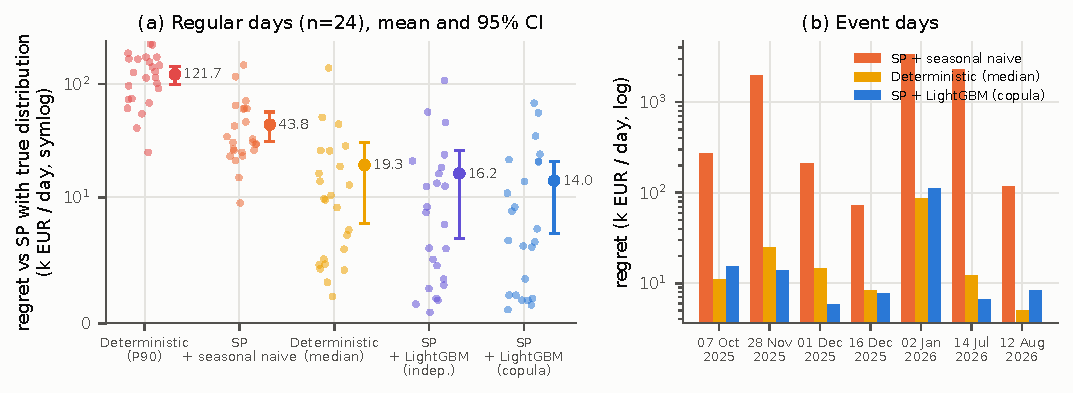
\includegraphics[width=\linewidth]{value_of_forecasts}
  \caption{(a) Daily regret on regular days (dots) with mean and 95\% confidence interval (symlog scale). (b) Event days: a forecast that does not know the retail calendar (seasonal naive) leaves millions of euros on the table on Black Friday, Prime Day and the Reyes peak.}
  \label{fig:value}
\end{figure}

\Cref{tab:value} and \cref{fig:value} support four conclusions.
\begin{enumerate}
  \item \textbf{Forecast quality dominates.} Planning with LightGBM instead of the true distribution costs \EUR{16.3}k per day on average (paired standard error \EUR{4.2}k; worse on all 31 days). This is about 0.6\% of the daily cost, or roughly \EUR{6}M per year at this volume, and it is an upper bound on what any further forecasting improvement could deliver. The seasonal-naive forecast has a regret of \EUR{44}k per day on regular days (\EUR{30}k more than LightGBM), and on event days it is catastrophic (\EUR{1.2}M per day on average): it schedules the capacity of an ordinary Friday for Black Friday.
  \item \textbf{Safety buffers are expensive.} Planning every series at its 90th percentile, a common heuristic, ignores that the 260 series do not peak together. It over-buys about 110 trucks and 50 crews per day and costs \EUR{96}k per day more than the stochastic program (paired $p<10^{-8}$), i.e.\ about \EUR{35}M per year.
  \item \textbf{The stochastic program beats the deterministic plan, modestly.} With the same LightGBM forecast, the SP with independent scenarios saves \EUR{2.9}k per day over the median plan (paired s.e.\ \EUR{1.1}k, $p=0.013$, better on 74\% of days). The SP with copula scenarios saves \EUR{3.8}k per day (s.e.\ \EUR{2.5}k, $p=0.14$). The gain is small because recourse is cheap in the base case; \cref{sec:flex} shows when it becomes large.
  \item \textbf{Correct joint calibration does not automatically pay.} The copula repairs the calibration of the national total (\cref{tab:scenarios}), but the paired cost difference to independent scenarios (\EUR{0.9}k per day) is not significant. The lesson is general: when recourse prices are nearly linear around the optimum, the plan is driven by the \emph{mean and the marginal quantiles at the critical ratio}, not by the shape of the joint distribution. Better forecasts of the level beat better forecasts of the dependence.
\end{enumerate}
